%Notes by Harsh Mistry 
%Econ 301
%Based on Template From  https://www.cs.cmu.edu/~ggordon/10725-F12/template.tex

\documentclass[twoside]{article}
\setlength{\oddsidemargin}{0.25 in}
\setlength{\evensidemargin}{-0.25 in}
\setlength{\topmargin}{-0.6 in}
\setlength{\textwidth}{6.5 in}
\setlength{\textheight}{8.5 in}
\setlength{\headsep}{0.75 in}
\setlength{\parindent}{0 in}
\setlength{\parskip}{0.1 in}
\usepackage{amsmath,amsfonts,graphicx, color}
\newcounter{lecnum}
\renewcommand{\thepage}{\thelecnum-\arabic{page}}
\renewcommand{\thesection}{\thelecnum.\arabic{section}}
\renewcommand{\theequation}{\thelecnum.\arabic{equation}}
\renewcommand{\thefigure}{\thelecnum.\arabic{figure}}
\renewcommand{\thetable}{\thelecnum.\arabic{table}}
\newcommand{\lecture}[4]{
   \pagestyle{myheadings}
   \thispagestyle{plain}
   \newpage
   \setcounter{lecnum}{#1}
   \setcounter{page}{1}
   
   
%Info Box 
   \begin{center}
   \framebox{
      \vbox{\vspace{2mm}
    \hbox to 6.28in { {\bf Econ 301 - Microeconomic Theory 2
	\hfill Winter 2018} }
       \vspace{4mm}
       \hbox to 6.28in { {\Large \hfill Lecture #1: #2  \hfill} }
       \vspace{2mm}
       \hbox to 6.28in { {\it Lecturer: #3 \hfill Notes By: #4} }
      \vspace{2mm}}
   }
   \end{center}
   
   \markboth{Lecture #1: #2}{Lecture #1: #2}



 
}

\renewcommand{\cite}[1]{[#1]}
\def\beginrefs{\begin{list}%
        {[\arabic{equation}]}{\usecounter{equation}
         \setlength{\leftmargin}{2.0truecm}\setlength{\labelsep}{0.4truecm}%
         \setlength{\labelwidth}{1.6truecm}}}
\def\endrefs{\end{list}}
\def\bibentry#1{\item[\hbox{[#1]}]}

\newcommand{\fig}[3]{
			\vspace{#2}
			\begin{center}
			Figure \thelecnum.#1:~#3
			\end{center}
	}
	
	\graphicspath{ {images/} }

\newtheorem{theorem}{Theorem}[lecnum]
\newtheorem{lemma}[theorem]{Lemma}
\newtheorem{ex}[theorem]{Example}
\newtheorem{proposition}[theorem]{Proposition}
\newtheorem{claim}[theorem]{Claim}
\newtheorem{corollary}[theorem]{Corollary}
\newtheorem{definition}[theorem]{Definition}
\newenvironment{proof}{{\bf Proof:}}{\hfill\rule{2mm}{2mm}}
\newcommand\E{\mathbb{E}}


%Start of Document 
\begin{document}

\lecture{2}{January 8, 2018}{Jean Guillaume Forand}{Harsh Mistry}

\section{Consumer Choice Continued}

\subsection{Feasible choices for consumers}
\textcolor{red}{In-Class Numbering : 1.1.2}

\begin{itemize}
\item A consumption bundle is a vector \(x = (x_1 , x_2) \in \mathbb{R}^2\) (i.e \(x_1, x_2 \geq 0\))
\end{itemize}

\begin{center}
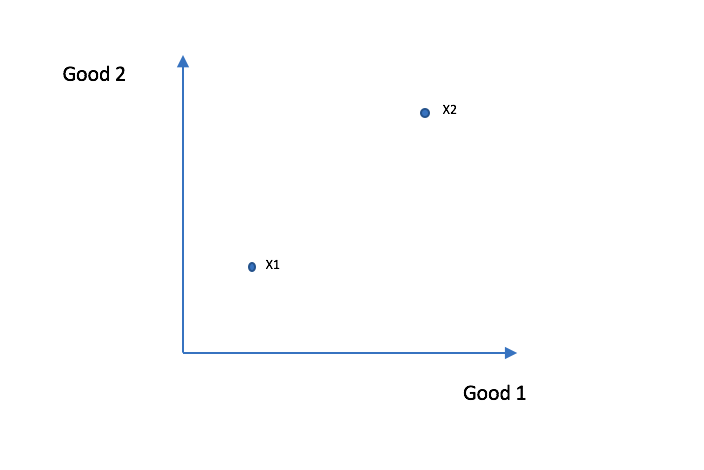
\includegraphics[scale=0.6]{1}
\end{center}

\begin{itemize}
\item Assume two goods for simplicity 
\item Assumes goods are only consumed in non-negative quantities 
\item Assumes units are arbitrarily divisible and any small quantity of good can be added to any bundle. Not essential, but allows for use of calculus methods. 
\item Not all consumptions bundles are feasible for the consumers, as the consumer purchases goods in markets 
\begin{itemize}
\item \underline{Market Prices} for two goods is a vector \(p = (p_1, p_2) \in \mathbb{R}^2\)
\item \underline{Income} of consumers is \(m > 0\) 
\end{itemize}
\end{itemize}

\begin{definition}
Given prices \(p\) and income \(m\), consumers \underline{budget set} is \[\beta = \{ (x_1, x_2) \in \mathbb{R}^2 \mid p_1 x_1 + p_2 x_2 \leq m \}\]
\end{definition}

\begin{center}
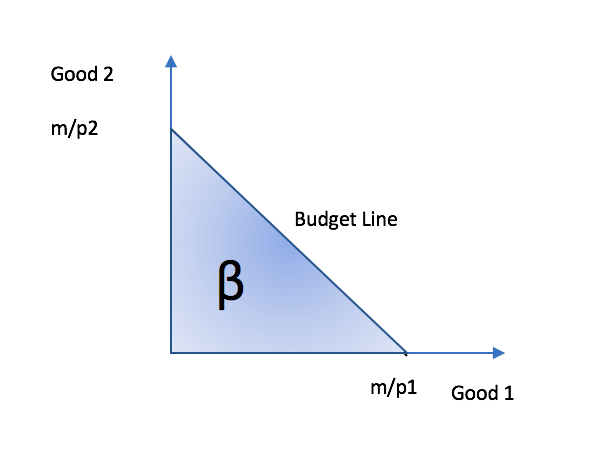
\includegraphics[scale=0.6]{2}
\end{center}

\begin{itemize}
\item Consumers need no find it optimal to exhaust his/her budget (i.e choose a consumption bundle on the budget line) 
\item Consumer is a \underline{price-taker} : Prices the consumer faces are independent of the consumption bundle  purchases
\item Appropriate assumptions for modelling large markets which no participants have significant market power
\item Slope of budget line \(\frac{-p_1}{p_2}\) is \underline{markets marginal rate of exchange} : rate at which market provides goods 2 against units of good 1
\end{itemize}

\begin{itemize}
\item Fix bundle \(x_1^*\), Let \(m^*\) be associated expenditure. 
\end{itemize}

\textbf{Question : } If a consumer wants to finance additional units of good 1 without increasing his expenditures, how much of good 2 must she supply to the market? 

\begin{itemize}
\item Have \(p_1x_1^* + p_2x_2^* = m^*\) 
\item Total derivatives of identity with respect to \(x_1\)
\[\begin{aligned}
p_1 \frac{dx_1^*}{dx_1^*} + p_2 \frac{dx_2^*}{dx_1^*} & = \frac{dm^*}{dx_1^*} \\
\frac{dx_2^*}{dx_1^*} & = \frac{-p_1}{p_2} 
\end{aligned}\]
\end{itemize}

\begin{itemize}
\item Price taking assumptions : market rate of exchange independent of \((x_1, x_2)\) 
\end{itemize}
\begin{ex} Rationing of good 1 there exists \(\bar{x_1}\), such that only bundles with \(x_1 \leq \bar{x_1}\) can be purchased

\end{ex}


\begin{center}
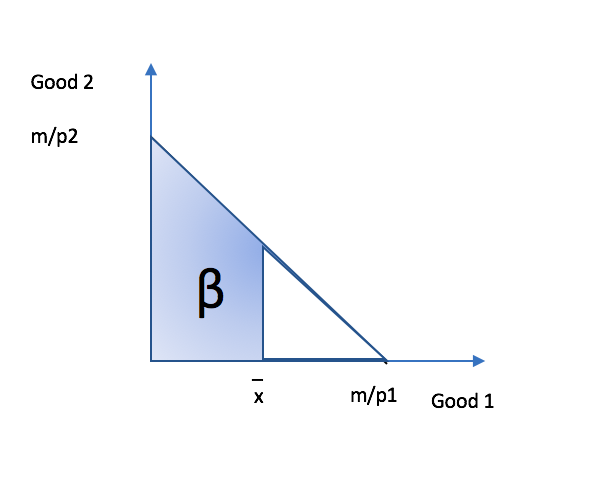
\includegraphics[scale=0.6]{3}
\end{center}

\subsection{Consumer Preferences}
\textcolor{red}{In-Class Numbering : 1.1.3}

\begin{itemize}
\item The consumer has goals or aspirations represented by a \underline{preference relation} \(\succeq\) over set of consumptions bundles \(\mathbb{R}^2_*\)
\item if \(x, y \in \mathbb{R}^2_*\) are such that \(x \succeq y\), we say that "x is weakly preferred to y"
\item \(\succeq\) is our primitive information about consumer which consists of pairwise comparisons of consumption bundles 
\item In principle, we can \underline{elicit} prederence by asking questions like "are you at least as well off with x as with y ?"
\item Do we prefer questions like : 
\begin{itemize}
\item Do you outright prefer x to y?
\item Are you indifferent between x and y? 
\end{itemize}
\end{itemize}
\end{document}





